\documentclass[TFM.tex]{subfiles}

\begin{document}


\chapter{Formality of Chain Operad of Little Disks}
POR AQUÍ TENGO QUE PONER LO DE EILENBERG-ZILBER, CUYA ASOCIATIVIDAD PERMITE QUE LA HOMOLOGÍA OBTENGA LA ESTRUCTURA DE OPERAD


EN GENERAL LO QUE PUEDA DE TAMARKIN


\url{https://ncatlab.org/nlab/show/augmentation}

\url{https://ncatlab.org/nlab/show/Drinfeld+associator}


PONER ALGO DE LO QUE SE VA A HACER EN ESTA SECCIÓN TIPO DICE QUÉ ES LA FORMALIDAD, DECIR QUE SE VA A PROBAR Y ALGO DE CÓMO (LOS PASOS) CITANDO QUE SIGO A TAMARKIN

\section{Braided operads and little disks operads}

We can substitute the group $\Sigma_n$ in the definition \ref{operadtop} by the braid group $B_n$, since there is a projection $B_n\to \Sigma_n$ with kernel $PB_n$ assigning to each braid $\sigma\in B_n$ the permutation that it induces on its endpoints. This way we obtain the notion of \emph{braided operad}. A \emph{topological $B_\infty$-operad} $X$ is defined as a braided operad such that all its spaces $X(n)$ are contractible and the braid group $B_n$ acts freely on $X(n)$. HABRÍA QUE COMPROBAR QUE ACTÚA LIBREMENTE EN EL RECUBRIDOR UNIVERSAL DE E2 (NO RECUERDO SI SE HACE EN BAR) If $X$ and $Y$ are topological $B_\infty$-operads, then so is $X\times Y$ and we have homotopi equivalences QUIZÁ EXPLICAR QUE EL PRODUCTO DE OPERADS ES OPERAD AUNQUE SEA EN EL CAPÍTULO DE OPERADS
\begin{equation}\label{projections}
p_1:X\times Y\to X;\ p_2:X\times Y\to Y,
\end{equation}
where $p_1$, $p_2$ are the projections. 

Given a topological $B_\infty$-operad $X$, the corresponding \emph{operad of little disks} is a symmetric operad $X'$ such that $X'(n)=X(n)/PB_n$ with the induced structure maps. The maps \ref{projections} guarantee that any two operads of little disks are connected by a chain of homotopy equivalencesHAY EQUIVALENCIA ENTRE LOS $X$ PERO LOS LITTLE DISKS SON LOS $X'$

 DEBERÍA COPIAR DE [6] LO DE CHAIN OF HOMOTOPY EQUIVALENCES


We now prove that the little disks operad defined in Section \ref{little} is a little disks operad in this sense. We'll make use of the following lemmas.

\begin{lemma}\label{contractible}
Let $(X,A)$ be a pair of topological spaces where $A$ is a contractible subspace  and let $p:\widetilde{X}\to X$ be a covering map. Then $p^{-1}(A)$ is a disjoint union of subspaces of $\widetilde{X}$, each of them mapped homeomorphically onto $A$ by $p$. 
\end{lemma}
\begin{proof}
In general, a fibre bundle over a contractible space is trivial \cite[Proposition 3.5]{bundle}, meaning that $p_X^{-1}(A)\cong A\times F_{x}$, where $F_x$ is the fibre over any point of $x\in A$. Since $p_X$ is a covering map, this fiber is discrete and we are done. 
\end{proof}

\begin{lemma}\label{lift}
Under the conditions of the previous leema, assume chosen base points $x\in A$ of $X$ and $y=f(x)\in B$ of $Y$ and choose lifts $\widetilde{A}$ of $A$ and $\widetilde{B}$ of $B$ given by the previous lemma. Choose also lifts $\widetilde{x}\in\widetilde{A}$ of $x$ and $\widetilde{y}\in\widetilde{B}$ of $y$. Then, if $f$ lifts to $\widetilde{f}:(\widetilde{X},\widetilde{x})\to (\widetilde{Y},\widetilde{y})$ as a map of based spaces, then $f$ lifts to $\widetilde{f}:(\widetilde{X},\widetilde{A})\to (\widetilde{Y},\widetilde{B})$ as a map of pairs. 
\end{lemma}
\begin{proof}
Since $A$ is contractible, it is path-connected, and so is $\widetilde{A}$. Then $\widetilde{f}(A)$ is a connected subspace of $\widetilde{Y}$ containing $\widetilde{y}$. Moreover, $p_Y(\widetilde{f}(A)=f(p_X(\widetilde{A}))=f(A)$, so $\widetilde{f}(\widetilde{A})$ is contained in $p_Y^{-1}(B)$, more specifically in the connected component containing $\widetilde{y}$, which is $\widetilde{B}$. Hence, $\widetilde{f}$ is actually a map of pairs.
\end{proof}

Now we follow the example 3.1 of \cite{bar} to prove:

\begin{prop}
The operad $E_2$ defined in Section \ref{little} is a little disks operad in the sense described above.
\end{prop} 
\begin{proof}
Let $\widetilde{E}_2(n)$ denote the universal cover of $E_2(n)$. We will dfine
an operad structure map and braid group actions on $\widetilde{E}_2$ by lifting them from the
structure map and symmetric group actions on $E_2$. Let $p:\widetilde{E}_2\to E_2$ the universal covering and let $E_1\subseteq E_2$ be the ``horizontal'' embedding of $E_1$ as little cubes of the form

DIBUJO DE FIEDEROWICZ PERO HECHO POR MÍ PORQUE LA FUENTE NO ES LA DE LATEX

ordered from left to right as shown. Note that the little cubes are homotopy equivalent to the little disks. By lemma \ref{contractible} and the fact that $E_1$ is contractible (see Section \ref{intervals}) we have that $p^{-1}(E_1(n))\subseteq\widetilde{E}_2(n)$ is a disjoint union of components, each homeomorphic to $E_1(n)$ via $p$. For each $n$, arbitrarily choose one these components and call it $\widetilde{C}_1(n)$. 

Now define the structure map $\widetilde{\gamma}$ for $\widetilde{E}_2$ to be the unique lifting 
\[
\begin{tikzcd}
\widetilde{E}_2(k)\times\widetilde{E}_2(j_1)\times\cdots\widetilde{E}_2(j_k) \arrow[r, "\widetilde{\gamma}", dashed] \arrow[d, "p"] & \widetilde{E}_2(j_1+\cdots+j_k) \arrow[d, "p"] \arrow[d] \\
E_2(k)\times E_2(j_1)\times\cdots E_2(j_1+\cdots+j_k) \arrow[r, "\gamma"]                                                                      & E_2(j_1+\cdots+j_k)                                     
\end{tikzcd}
\]
which takes $\widetilde{E}_1(k)\times\widetilde{E}_1(j_1)\times\cdots\widetilde{E}_1(j_k)$ to $\widetilde{E}_1(j_1+\cdots+j_k)$. The existence and uniqueness of this map is guaranteed by lemma \ref{lift} since $\gamma$ clearly takes the embedding $E_1(k)\times E_1(j_1)\times\cdots E_1(j_k)$ to the embedding of $E_1(j_1+\cdots+j_k)$. Here we're implicitly making use of the theory of covering spaces, in particular the lifting properties of the universal cover, see Section 1.3 of \cite{HA} for a complete treatment of the subject. Also recall that the product of covering spaces is a covering space of the product (Exercise 2 from page 79 of \cite{HA}).

CONTINUAR CON LA ACCIÓN (SACAR EL DIBUJO DEL GENERADOR DE ARTIN DE MI TFG)

EL EJEMPLO DE FIEDEROWICZ CON LA PRUEBA DEL EJERCICO QUE ME PUSO MURO (A infinito significa que los espacios del operad son contráctiles, esto para el caso sin acción del grupo simétrico, que es el que usa Fiedorowicz. Con acción significa que cada componente conexa es contráctil, pero en cualquier caso C1 es contráctil \url{https://en.wikipedia.org/wiki/A\%E2\%88\%9E-operad}) 

\end{proof}



The functor of singular chains $C_*^{sing}:\Top\to \Ch$ has a natural tensor (lax monoidal) structure given by the Eilenberg-Zilber map $EZ:C_*^{sing}(X)\otimes C_*^{sing}(Y)\to C_*^{sing}(X\times Y)$. Therefore, for a topological operad $O$, the coleccion $C_*^{sin}(O(*))$ has a structure of a dg-operad. The structure map of the $i$-th insertion is 
\[
C_*^{sing}(O(n))\otimes C_*^{sing}(O(m))\xrightarrow{EZ} C_*^{sing}(O(n)\times O(m))\xrightarrow{\circ_{i*}} C_*^{sing}(O(n+m-1)),
\]
where $\circ_i$ is the structure map of the $i$-th insertion in $O$. We need to check that the associativity axiom of the operad structure still holds after applyin the Eilenberg-Zilber map. In order to prove it, we use its explicit formulation \cite{EZ}

\url{https://ncatlab.org/nlab/show/Eilenberg-Zilber+map}
HACER LA PRUEBA 

For a little disks operad $X$ consider the operad $E_2(X)=C_*^{sing}(X)$ CREO QUE DEBERÍA CAMBIAR LA NOTACIÓN. Any two such operads are quasi-isomorphic PONER EN ALGÚN LADO LO DE CHAIN OF QUASI-ISOMORPHISM DE [6]. In particular, the homology operad of any $E_2(X)$ is the operad $e_2$ CAMBIAR ESTA NOTACIÓN TAMBIÉN controlling Gerstenhaber algebras. Our goal in this chapter is to show the following.

\begin{thm}
Any operad $E_2(X)$ is quasi-isomorphic to its homology operad $e_2$.
\end{thm}

It suffices to prove this theorem only for one operad $X$ of little disks since they are all homotopy equivalent. We will prove it for the one defined in the next section.

\section{The category operad $PaB_n$}

We're going to define a category operad $PaB_n$. Let $B_n$ the group of braids on $n$ strands and $PB_n$ the group of pure braids on $n$ strand. Let $\Sigma_n$ the symmetric group and let $p:B_n\to \Sigma_n$ be the canonical projection with kernel $PB_n$. We assume that the strands of any braid are numbered in the order determined by their origins. 

The objects of the category $PaB_n$ are parenthesized permutations of the set $\{1,\dots, n\}$ (that is pairs $(\sigma,\pi)$, where $\sigma\in\Sigma_n$ and $\pi$ is a parenthesizing of the non-associative product of $n$ elements). The morphisms between $(\sigma_1,\pi_1)$ and $(\sigma_2,\pi_2)$ are such braids in $B_n$ that any strand joins an element of $\sigma_1$ with the same element of $\sigma_2$, in other words, $\Hom((\sigma_1,\pi_1),(\sigma_2,\pi_2))=p^{-1}(\sigma_2^{-1}\sigma_1)$. The composition law is induced from the one on $B_n$. The symmetric group $\Sigma_n$ acts on $PaB_n$ via renumbering the objects: $\tau(\sigma,\pi)=(\tau\sigma,\pi)$ for $\tau\in\Sigma_n$ and $(\sigma,\pi)\in PaB_n$. 

%\url{https://ncatlab.org/nlab/show/parenthesized+braid+operad}

The collection of categories $PaB_n$ form an operad. Indeed, the collection of objects $PaB_*$ forms an operad in the category of magmas (sets generated by one non-commutative operation). COMENTAR LA INSERCIÓN EN OBJETOS, SERÍA SIMPLEMENTE METER LOS NÚMEROS O PALABRAS DENTRO, CREO QUE AQUÍ BASTARÍA RENUMERAR A PARTIR DEL $N+1$ PORQUE NO HACE FALTA CONTINUIDAD Let us describe the structre map $\circ_k$ of the insertion into the $k$-th position on the level of morphisms. Suppose we insert $y:(\sigma_1,\pi_1)\to (\sigma_2,\pi_2)$ into $x:(\sigma_3,\pi_3)\to(\sigma_4,\pi_4)$. We replace the strand number $\sigma^{-1}_3(k)$ of the braid $x$ by the braid $y$ made very narrow, as shown in the picture.

\begin{figure}[h!]
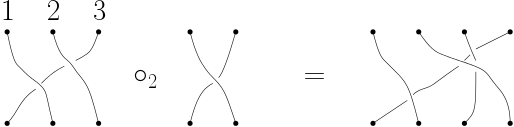
\includegraphics[scale=0.7]{Imagenes/insercion.png}
\caption{Insertion of the right braid into the second strand of the left braid.}
\end{figure}

\subsection{Operad of classifying spaces}

We have the functor of taking the nerve $N:\Cat\to\SSet$ and the functor of topological realization $|\ |:\SSet\to \CW$. One can easily check that the nerve functor behaves well with respect to the symmetric monoidal structure. Since the nerve $PaB_n$ is countable, the realization also behaves well with its symmetric monoidal structure by \ref{countable}. Let us check that the collection of cellular complexes $X_n=|N(PaB_n)|$ forms a cellular operad. Let $PaB_n'$ be the category whose objects are pairs $(x,y)$, where $x$ belongs to the braid group $B_n$ and $y$ is a parenthesizing of the non-associative product of $n$ elements, and there is a unique morphism between any two objects. We have a free left action of $B_n$ on $PaB_n':(x,y)\to (gx,y)$ and a braided operad structre on $PaB_*'$ (the structre maps are defined similarly to $PaB_n$ COMPROBARLO). We have to show that the corresponding operad of classifying spaces is a topological $B_\infty$-operad and that the corresponding little disks operad is isomorphic to $X_*$ HACERLO.

Consider the corresponding chain operad. Let $C_*(PaB_n)$ be the chain complex over $\Q$ of $NPaB_n$ as a simplicial set. The collection $C_*(NPaB_n)$ forms a dg-operad (via the Eilenberg-Zilber map). We have a canonical quasi-isomorphism of operads $C_*(PaB_*)\to C_*^{sing}(|NPaB_*|)$ (just like the quasi-isomorphism between simplicial homology and singular homology). Therefore is suffices to construct a quasi-isomorphism of $C_*(PaB_*)$ and $e_2$ CAMBIAR NOTACIÓN.
\end{document}
